%! Author = joshu
%! Date = 9/8/20

% Preamble
\documentclass[11pt]{article}
\title{Week 7-1 notes, Series with Negative Terms}
\author{Joshua Petitma}
\date{9/28/2020}
\renewcommand{\thesubsection}{\thesection.\alph{subsection}}
\newcommand{\bv}[2]{\big\vert_{#1}^{#2}}
\usepackage{xcolor,cancel}

\newcommand\hcancel[2][black]{\setbox0=\hbox{$#2$}%
\graphicspath{{images/}}
\rlap{\raisebox{.45\ht0}{\textcolor{#1}{\rule{\wd0}{1pt}}}}#2}
\usepackage{hyperref}
% Packages
\usepackage{amsmath}
\usepackage{amssymb}
\usepackage{graphicx}

% Document
\begin{document}
    \part[Video 1, Series with Negative Temrs]{The Alternating Series Test}
    \section[The Alternating Series Test]{The Alternating Series Test}
    \subsection*{Definition: An alternating series is a series with terms that alternate between positive and negative
    (every other term)}

    \section*{Examples:}
    \label{sec:Examples}
    \subsection[Examples.1]{}
    \label{subsec:Examples1}
    \begin{flalign*}
        \sum_{k=1}^{\infty}{\frac{\boxed{(-1)^{k-1}}}{k}} &&
    \end{flalign*}

    \subsection[Examples.2]{}
    \label{subsec:Examples2}
    \begin{flalign*}
        \sum_{k=1}^{\infty} \frac{\boxed{(-1)^k k}}{k^3 + 1} &&
    \end{flalign*}

    \subsection[Examples.3]{}
    \label{subsec:Examples3}
    \begin{flalign*}
        \sum_{k=1}^{\infty} \frac{\boxed{(-1)^{k+1}}}{2^k + 1} &&
    \end{flalign*}

    Odd indexed Terms are negative (1.b) Even indexed Terms are negative (1.a and 1.c)

    \paragraph[para]{}
     For series with positive terms, $S_n$ is increasing.

    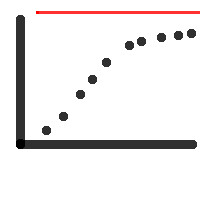
\includegraphics{week7graph.jpg}

    This is not the case with alternating series

    \section[Alternating Harmonic Series] {Example: Alternating Harmonix Series}
    \begin{flalign*}
        \sum_{k=1}^{\infty} \frac{(-1)^{k-1}}{k} && \\
        S_1 &= 1 \\
        S_2 &= 1 + (-\frac{1}{2}) = \frac{1}{2} \\
        S_3 &= 1 + (-\frac{1}{2}) = \frac{1}{2} + \frac{1}{3} = \frac{5}{6}\\
        S_4 &= 1 + (-\frac{1}{2}) = \frac{1}{2} + \frac{1}{3}  + (-\frac{1}{4}) + \frac{14}{24}
    \end{flalign*}
    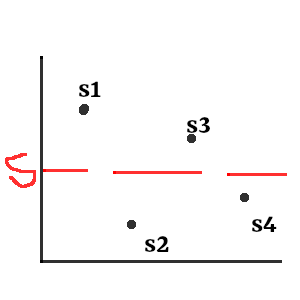
\includegraphics{./week7graph2.png}

    Because the $1^st$ is positive

    $S_1 > S_# > S_5 > \dots$

    $S_2 < S_4 < S_6 < \dots$
    \paragraph[]{Alternating Series:}Consider the alternating series
    $ \sum_{k=1}^{\infty} a_k$ where
    \begin{flalign*}
        a_k &= (-1)^k b_k\ \text{or}&&\\
        &= (-1)^{k-1}b_k \\
        &= (-1)^{k+1}b_k \\
    \end{flalign*}
    If both
    \begin{enumerate}
        \item $ \lim_{k\to\infty} b_k = 0 $ AND
        \item $ b_{k+1} < b_k$ (decreasing)
    \end{enumerate}
    Then the alternating series converges

    \part[Video 2, Series with Negative Terms] {Alternating Series Test Examples}
    \section* {Examples:}
    \subsection[Example.1]{}
    \label{subsec:Example1}
    \begin{flalign*}
        \sum_{k=1}^{\infty} \frac{(-1)^{k-1}}{k}
    \end{flalign*}
    (i) $ \lim_{k\to\infty} \frac{1}{k} = 0$ \\
    (ii) $ \frac{1}{k+1} < \frac{1}{k}$

    So The series converges by Alternating Series Test (AST)

    \subsection[Example.2]{}
    \label{subsec:Example2}
    \begin{flalign*}
        \sum_{k=1}^{\infty} \frac{(-1)^k \sqrt{k}}{k+4} &&\\
        (i)  &\lim_{k\to\infty} \frac{\sqrt{k}}{k+4} &&\\
        (ii) & \frac{\sqrt{k+1}}{(k+1) + 4} < \frac{\sqrt{k}}{k+4}\\
        &= \frac{k+1}{(k+5)^2} < \frac{k}{(k+4)^2} \\
        &= (k+1)(k^2 + 8k + 16) < k(k^2 + 10k + 25) \\
        &= \hcancel{k^3} + 8k^2 + 16k + k^2 + 8k + 16 < \hcancel{k^3} + 10k^2 + 25k \\
        &= 16 < k^2 + k \\
    \end{flalign*}
    This holds for the $k \geq 4$, This suffices.
    We just have to prove that it holds true for all values of $k$ after some fixed value.
    \\\fbox{This converges by AST}

    \subsection[Example.3]{$ \sum_{k=1}^{\infty}  \frac{(-1)^k k}{k+3}$}
    \label{subsec:Example3}
    \begin{flalign*}
        &(i) \lim_{k\to\infty}\frac{k}{k+3} = 1 \neq 0 &&\\
    \end{flalign*}
    The series \fbox{diverges} by the Test for Divergence

    \subsection[Example.3]{}Does the series $ \frac{1}{2^2} - \frac{1}{2^3} + \frac{1}{3^2} - \frac{1}{3^3} +
    \frac{1}{4^2} - \frac{1}{4^3} + \dots$ converge?
    \label{subsec:Example3}
    \begin{flalign*}
        &(i) \lim_{k\to\infty}b_k = 0\ \text{\checkmark}\\
        \text{but} \\
        &\hcancel[red]{(ii)} b_k+1 < b_k\ \text{X}
    \end{flalign*}
    Can't use AST\\
    This can be written as \\
    $ \sum_{k=2}^{\infty} \frac{1}{k^2} - \sum_{k=2}^{\infty}\frac{1}{k^3} $
    \\ Both of these converge (p-series, $ p> 1$) So the original series converges

    \part[Video 3, Absolute vs. Conditional Convergence]{Absolute vs. Conditional Convergence}
    \section*{Example:}
    $ \sum_{k=1}^{\infty} \frac{\sin(k)}{k^2}$ This series has negative terms, but is not alternating

    \section[Absolute Convergence Theoriem]{Absolute Convergence Theorem}
    if $\sum_{k=1}^{\infty} |a_k|$ converges, then $\sum_{k=1}^{\infty} a_k$ converges.
    \\\\
    \textbf{Important:} Not an if and only if statement
    \\
    \begin{flalign*}
        \sum_{k=1}^{\infty}  \frac{(-1)^{k-1}}{k}\ \text{converges, but} \\
        \sum_{k=1}^{\infty} |\frac{(-1^{k-1})}{k}| = \sum_{k=1}^{\infty} \frac{1}{k}\ \text{diverges}
    \end{flalign*}

    \subsection[Example.2]{$ \sum_{k=1}^{\infty} \frac{\sin(k)}{k^2}$}
    \label{subsec:Example2}
    \begin{flalign*}
        \sum_{k=1}^{\infty} |\frac{sin(k)}{k^2}| \leq \sum_{k=1}^{\infty}  \frac{1}{k^2}\ \text{which converges}
    \end{flalign*}
    So $ \sum_{k=1}^{\infty} |\frac{\sin(k)}{k^2}|$ \\
    So $ \sum_{k=1}^{\infty}  \frac{\sin(k)}{k^2}$ \fbox{converges} by Abs. cmv. thm.
\end{document}
